\documentclass[border=10pt]{standalone}
% Shared style for the EMONI diagrams. Build: tectonic <file>.tex, then pdftocairo -svg.
\usepackage{fontspec}
\setmainfont{FiraSans}[Extension=.otf,UprightFont=*-Regular,BoldFont=*-SemiBold,ItalicFont=*-Italic,BoldItalicFont=*-SemiBoldItalic]
\setmonofont{FiraMono}[Extension=.otf,UprightFont=*-Regular,BoldFont=*-Medium,Scale=0.9]
\usepackage{tikz}
\usetikzlibrary{arrows.meta,positioning,shapes.geometric,shapes.misc,calc,fit,backgrounds}
\definecolor{eg}{HTML}{11903B}   % EMONI green
\definecolor{egl}{HTML}{E8F7EE}
\definecolor{eb}{HTML}{2A78D6}   % blue
\definecolor{ebl}{HTML}{EAF2FC}
\definecolor{eo}{HTML}{D9631E}   % orange
\definecolor{eol}{HTML}{FDF0E7}
\definecolor{ep}{HTML}{7C4DCC}   % purple
\definecolor{epl}{HTML}{F2ECFB}
\definecolor{er}{HTML}{C5221F}   % red
\definecolor{erl}{HTML}{FCEAEA}
\definecolor{ink}{HTML}{1F2328}
\definecolor{mute}{HTML}{59636E}
\definecolor{line}{HTML}{D0D7DE}
\tikzset{
  every node/.style={text=ink,font=\small},
  >={Stealth[length=2.4mm]},
  % sequence diagrams
  life/.style={draw=line,dashed,thick},
  head/.style={draw=#1,fill=#1!8,rounded corners=3pt,minimum width=27mm,minimum height=11mm,align=center,font=\small\bfseries,thick},
  act/.style={draw=#1,fill=#1!18,minimum width=2.2mm},
  msg/.style={->,thick,draw=ink},
  ret/.style={->,dashed,draw=mute},
  mlabel/.style={font=\footnotesize,fill=white,inner sep=1.5pt,align=center},
  note/.style={draw=#1,fill=#1!8,rounded corners=2pt,font=\footnotesize,align=left,inner sep=4pt},
  frag/.style={draw=mute,rounded corners=2pt},
  fraglabel/.style={draw=mute,fill=white,font=\footnotesize\bfseries,inner sep=2.5pt,anchor=north west},
  % activity diagrams
  start/.style={circle,fill=ink,minimum size=4mm,inner sep=0},
  stop/.style={circle,draw=ink,thick,minimum size=5mm,inner sep=0,path picture={\fill[ink] (path picture bounding box.center) circle (1.4mm);}},
  step/.style={draw=#1,fill=#1!8,rounded corners=5pt,thick,minimum height=9mm,minimum width=40mm,align=center,font=\small},
  step/.default=eg,
  dec/.style={diamond,aspect=2.2,draw=ink,fill=white,thick,inner sep=1.5pt,align=center,font=\footnotesize},
  flow/.style={->,thick,draw=ink},
  guard/.style={font=\footnotesize\itshape,text=mute,fill=white,inner sep=1.5pt},
  lane/.style={draw=line,fill=#1,rounded corners=4pt},
  lanetitle/.style={font=\small\bfseries,text=mute},
}

% Activity: how a problem in the field is tracked, debugged, fixed and verified.
\begin{document}
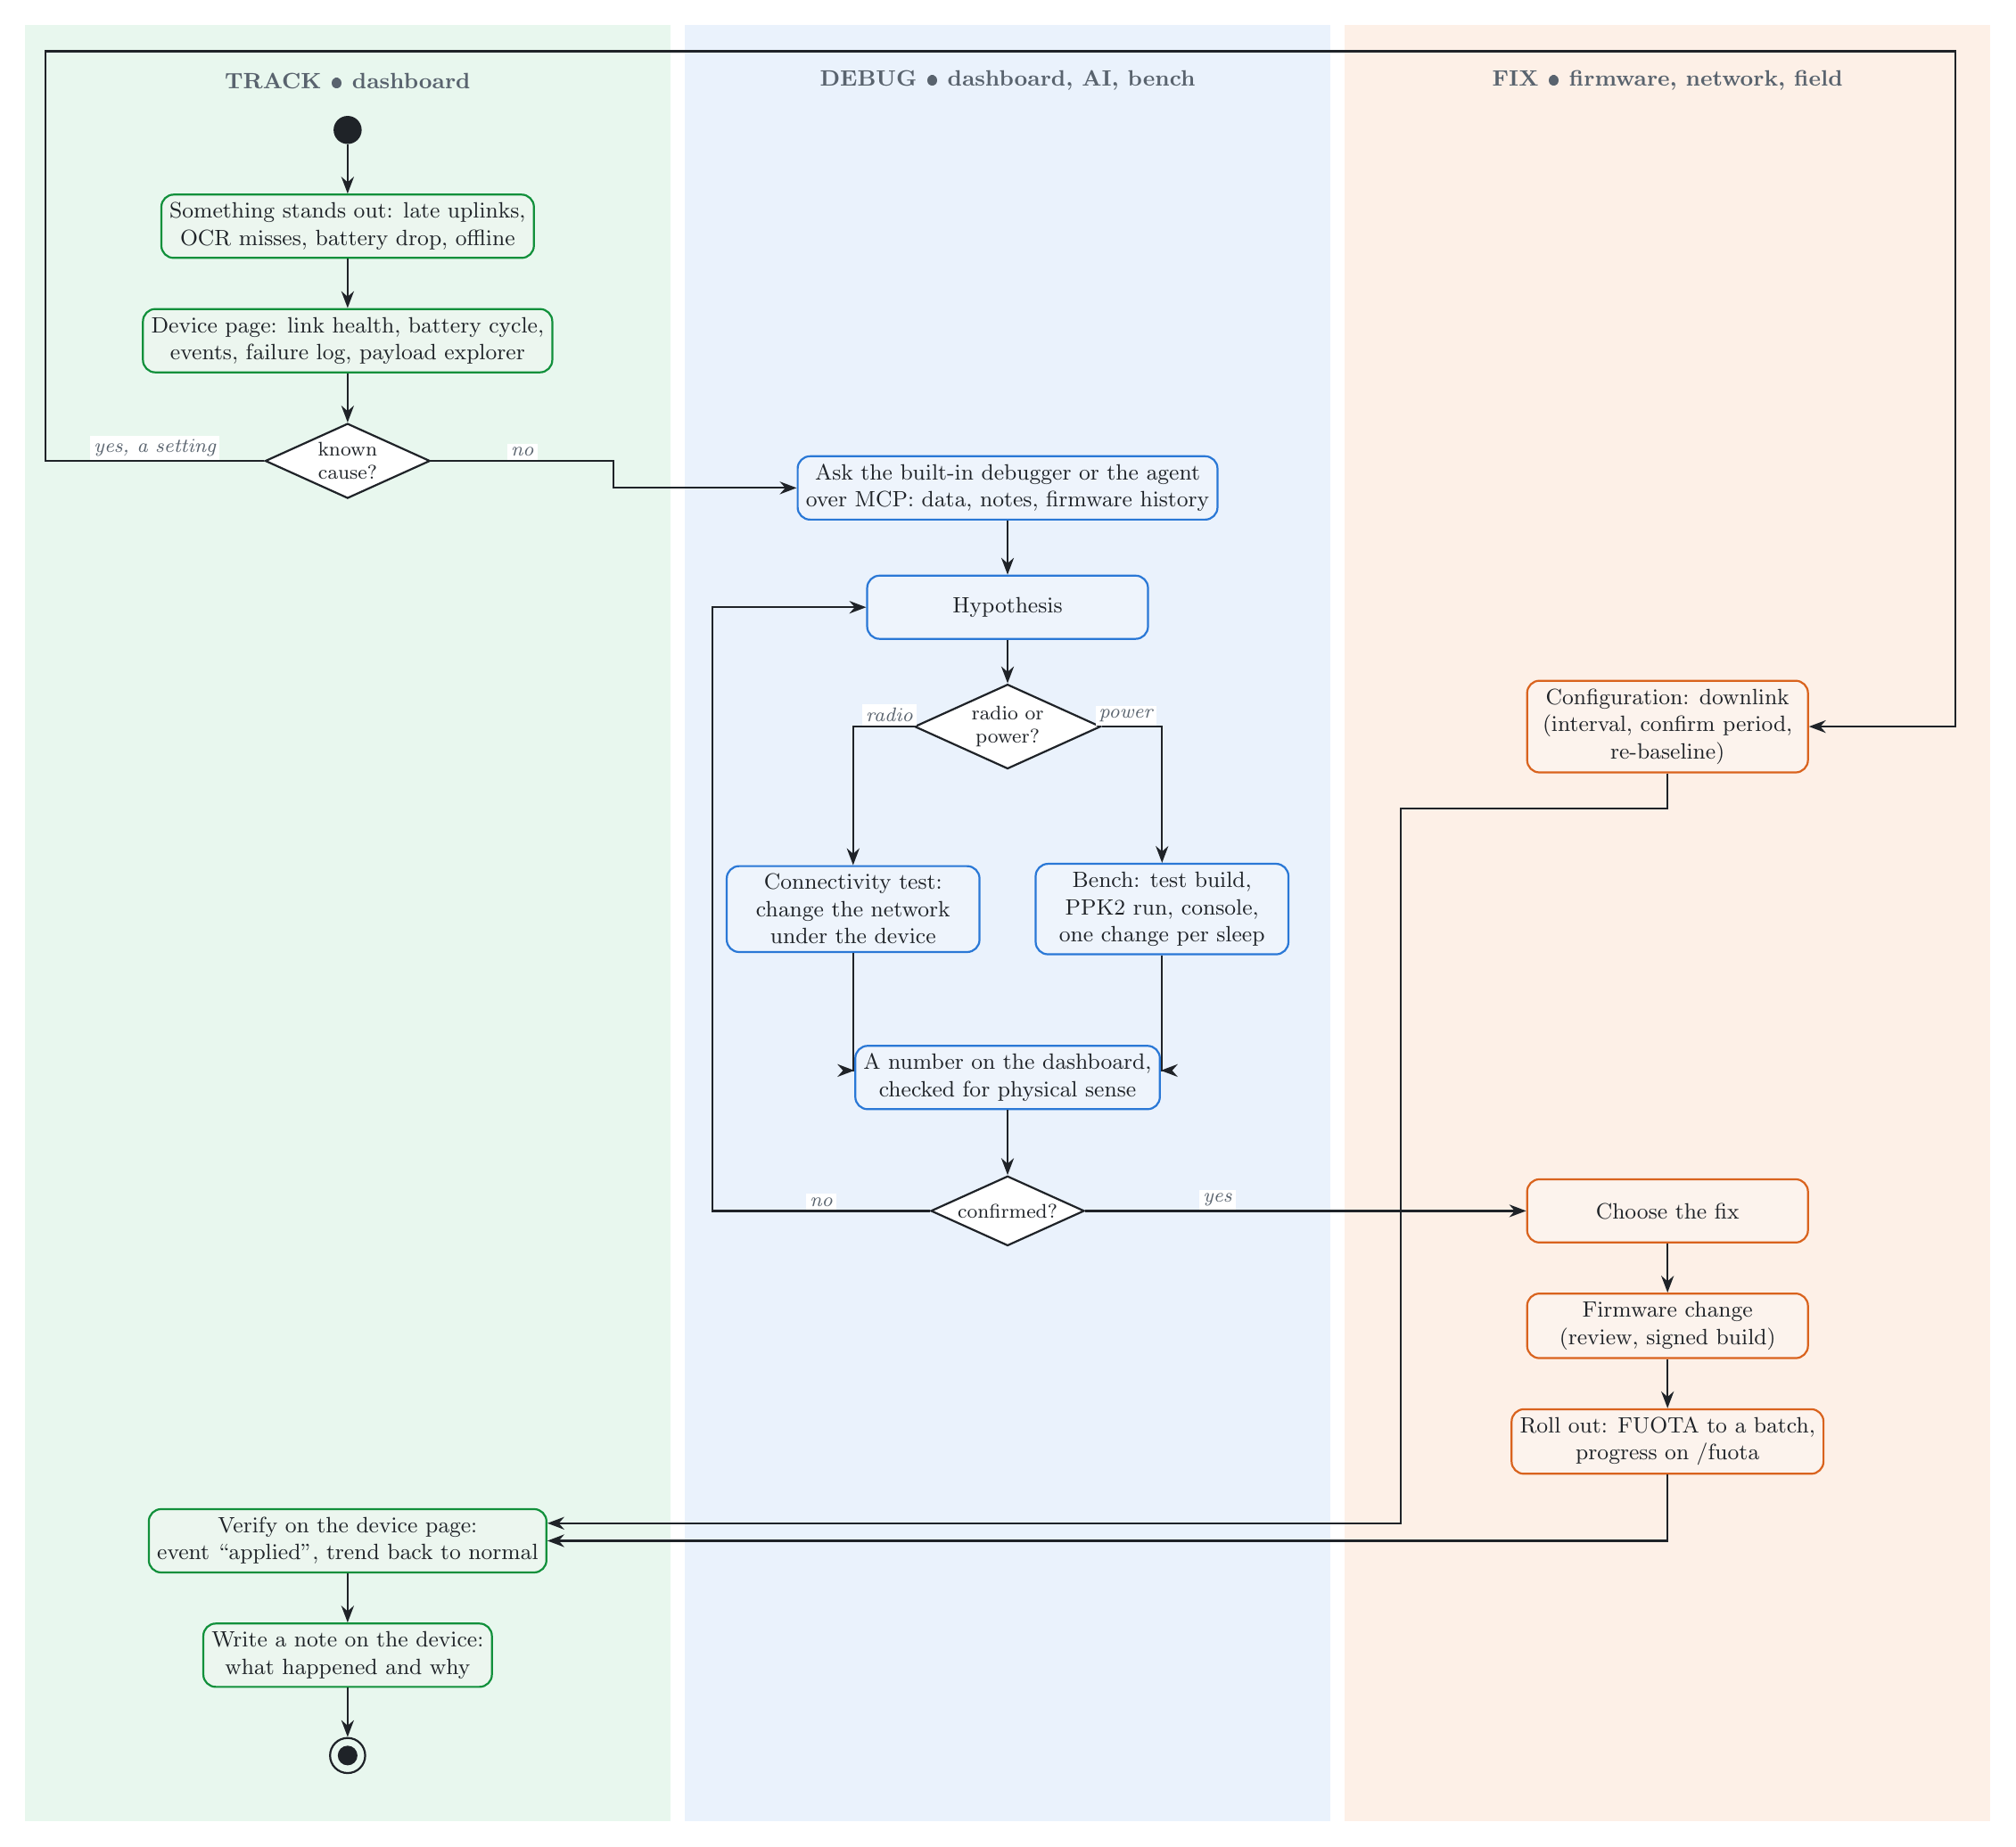
\begin{tikzpicture}[node distance=7mm and 10mm]
% lanes
\fill[egl] (-4.6,1.0) rectangle (4.6,-24.6);
\fill[ebl] (4.8,1.0) rectangle (14.0,-24.6);
\fill[eol] (14.2,1.0) rectangle (23.4,-24.6);
\node[lanetitle] at (0,0.2) {TRACK \textbullet{} dashboard};
\node[lanetitle] at (9.4,0.2) {DEBUG \textbullet{} dashboard, AI, bench};
\node[lanetitle] at (18.8,0.2) {FIX \textbullet{} firmware, network, field};
\node[start] (s) at (0,-0.5) {};
\node[step,below=of s] (sym) {Something stands out: late uplinks,\\OCR misses, battery drop, offline};
\node[step,below=of sym] (look) {Device page: link health, battery cycle,\\events, failure log, payload explorer};
\node[dec,below=of look] (known) {known\\cause?};
\node[step=eb] (ai) at (9.4,-5.6) {Ask the built-in debugger or the agent\\over MCP: data, notes, firmware history};
\node[step=eb] (hyp) at (9.4,-7.3) {Hypothesis};
\node[dec] (where) at (9.4,-9.0) {radio or\\power?};
\node[step=eb,minimum width=36mm] (ct) at (7.2,-11.6) {Connectivity test:\\change the network\\under the device};
\node[step=eb,minimum width=36mm] (pw) at (11.6,-11.6) {Bench: test build,\\PPK2 run, console,\\one change per sleep};
\node[step=eb] (num) at (9.4,-14.0) {A number on the dashboard,\\checked for physical sense};
\node[dec] (conf) at (9.4,-15.9) {confirmed?};
\node[step=eo] (kind) at (18.8,-15.9) {Choose the fix};
\node[step=eo,below=of kind] (fw) {Firmware change\\(review, signed build)};
\node[step=eo,below=of fw] (ota) {Roll out: FUOTA to a batch,\\progress on /fuota};
\node[step=eo] (cfg) at (18.8,-9.0) {Configuration: downlink\\(interval, confirm period,\\re-baseline)};
\node[step=eg] (ver) at (0,-20.6) {Verify on the device page:\\event ``applied'', trend back to normal};
\node[step=eg,below=of ver] (note) {Write a note on the device:\\what happened and why};
\node[stop,below=of note] (e) {};
\draw[flow] (s)--(sym); \draw[flow] (sym)--(look); \draw[flow] (look)--(known);
\draw[flow] (known.east) -- node[guard,above]{no} ++(2.6,0) |- (ai.west);
\draw[flow] (known.west) -- node[guard,above]{yes, a setting} (-4.3,0 |- known.west) -- (-4.3,0.62) -- (22.9,0.62) |- (cfg.east);
\draw[flow] (ai)--(hyp); \draw[flow] (hyp)--(where);
\draw[flow] (where.west) -| node[guard,above,pos=0.2]{radio} (ct.north);
\draw[flow] (where.east) -| node[guard,above,pos=0.2]{power} (pw.north);
\draw[flow] (ct.south) |- ($(num.west)+(0,0.1)$);
\draw[flow] (pw.south) |- ($(num.east)+(0,0.1)$);
\draw[flow] (num)--(conf);
\draw[flow] (conf.east) -- node[guard,above,pos=0.3]{yes} (kind.west);
\draw[flow] (conf.west) -- node[guard,above]{no} (5.2,0 |- conf.west) |- (hyp.west);
\draw[flow] (kind)--(fw); \draw[flow] (fw)--(ota);

\draw[flow] (ota.south) |- (ver.east);
\draw[flow] (cfg.south) -- ++(0,-0.5) -| (15.0,-14.6) |- ($(ver.east)+(0,0.25)$);
\draw[flow] (ver)--(note); \draw[flow] (note)--(e);
\end{tikzpicture}
\end{document}
